\documentclass[conference]{IEEEtran}
\IEEEoverridecommandlockouts
\usepackage{cite}
\usepackage{amsmath,amssymb,amsfonts}
\usepackage{graphicx}
\usepackage{textcomp}
\usepackage{xcolor}
\usepackage{booktabs}
\usepackage{url}

% Red placeholders: every one of these must be replaced by a number from
% results/paper_tables (merge_results.py) or results/deep44 (analyze_44.py).
\newcommand{\PH}[1]{\textcolor{red}{[#1]}}

\begin{document}

\title{Does Condition Normalisation Help Autoencoder Fault Detection? A Leakage-Safe Evaluation on All 95 CARE-to-Compare Wind Turbine Datasets}

\author{
\IEEEauthorblockN{N Ananth}
\IEEEauthorblockA{\textit{Dept. of Artificial Intelligence and Machine Learning}\\
\textit{RV College of Engineering}\\
Bengaluru, India\\
nananth.ci25@rvce.edu.in}
\and
\IEEEauthorblockN{Roshan Kalirajan}
\IEEEauthorblockA{\textit{Dept. of Computer Science (Data Science)}\\
\textit{RV College of Engineering}\\
Bengaluru, India\\
roshankalirajan.cd25@rvce.edu.in}
\and
\IEEEauthorblockN{Samarth B N}
\IEEEauthorblockA{\textit{Dept. of Electronics and Communication Engineering}\\
\textit{RV College of Engineering}\\
Bengaluru, India\\
samarthbn.ec25@rvce.edu.in}
\and
\IEEEauthorblockN{Veena Gadad\textsuperscript{*}}
\IEEEauthorblockA{\textit{Dept. of Computer Science and Engineering}\\
\textit{RV College of Engineering}\\
Bengaluru, India\\
veenagadad@rvce.edu.in}
}

\maketitle

\begin{abstract}
Autoencoders trained on normal operation are a common way to flag faults in wind turbine SCADA data, but their reconstruction error also follows wind and load. A frequent remedy is to model the error that operating conditions explain and score only the excess. We test this remedy, together with causal smoothing, on all 95 datasets of the CARE-to-Compare benchmark (three farms, 45 faults, 50 normal periods). All settings were fixed before testing; every variant is run with three seeds and compared with Isolation Forest, PCA and a 3$\sigma$ rule using the benchmark's CARE score, with a paired bootstrap over datasets. The plain autoencoder scores $0.584\pm0.002$ and the full pipeline $0.592\pm0.004$, against 0.5 for random predictions and 0.66 for a per-farm tuned autoencoder in the benchmark paper. Condition normalisation alone lowers the score to 0.568: it cuts false alarms but also hides part of the fault signal. None of the autoencoder variants differ significantly from each other or from PCA (0.598). The one clear gain is for Isolation Forest, where normalisation plus smoothing adds 0.048 (95\% CI 0.003 to 0.094). Plant-area attribution names the operator's root cause first in up to 37\% of 40 labelled faults, against 12\% for a random ranking and 30\% for always naming the commonest area. \PH{One sentence from v3: leave-one-farm-out tuning and the conditional autoencoder.} A causal health index with a time-to-threshold band and a Unity playback are shown on two faults, one missed and one detected.
\end{abstract}

\begin{IEEEkeywords}
offshore wind, SCADA, autoencoder, normal behaviour model, CARE score, anomaly attribution, predictive maintenance, digital twin
\end{IEEEkeywords}

\section{Introduction}
Offshore plants often produce more energy than onshore machines of similar rating, but a repair visit needs a vessel, a weather window, and spare parts \cite{r5,r8}. Reactive repair waits for a stop, and calendar-based repair visits the machine whether it needs work or not \cite{r3,r5}. A middle path is to read the SCADA archive, mark unusual behaviour early, and only then place a work order \cite{r20}.

Normal behaviour models do this by learning what the sensors look like when the turbine is healthy and flagging departures from it \cite{r21,r22,r23}. Autoencoders are popular because one network can watch hundreds of channels at once \cite{r10,r11,r25}. Their reconstruction error, however, depends on the operating point: a healthy turbine at rated power and one idling in light wind do not have the same typical error. The benchmark paper we use handles this with an adaptive threshold, a second network that predicts the expected error, tuned per farm \cite{r12}, and a conditional autoencoder that takes operating conditions as input has been proposed for district heating \cite{r19}. Whether such corrections help on a large, labelled set of real faults, and by how much once tuning is taken out of the comparison, is less clear. Many published results also come from one turbine, one fault, or a random split that places fault rows in the training set \cite{r12,r28,r29}.

An earlier version of this work had exactly those problems: it trained on a file that already contained the fault, reported no detection rates, used a sigmoid output on standardised data and compared against nothing. CSITSS reviewers rightly asked for a clean split, precision and false-alarm rates, baselines, repeated runs, justified thresholds and an uncertainty band on the life estimate. This paper answers each point and reports the outcome even where it is negative. Its contributions are:
\begin{itemize}
\item a leakage-safe evaluation of condition normalisation and causal smoothing on all 95 CARE-to-Compare datasets, with settings fixed in advance, three seeds, three baselines, an ablation of every step and a paired bootstrap over datasets;
\item \PH{v3: leave-one-farm-out tuning of threshold and alarm counter, and a conditional autoencoder}, which show how much of the gap to the tuned benchmark result comes from tuning;
\item a check of plant-area attribution against operator fault notes in three farms, against random, majority-class and model-free floors;
\item a causal health index and time-to-threshold estimate with a 95\% band, a gate sensitivity study instead of hand-picked weights, and a Unity playback of measured values.
\end{itemize}

\begin{figure*}[t]
\centering
\IfFileExists{figures/pipeline.png}{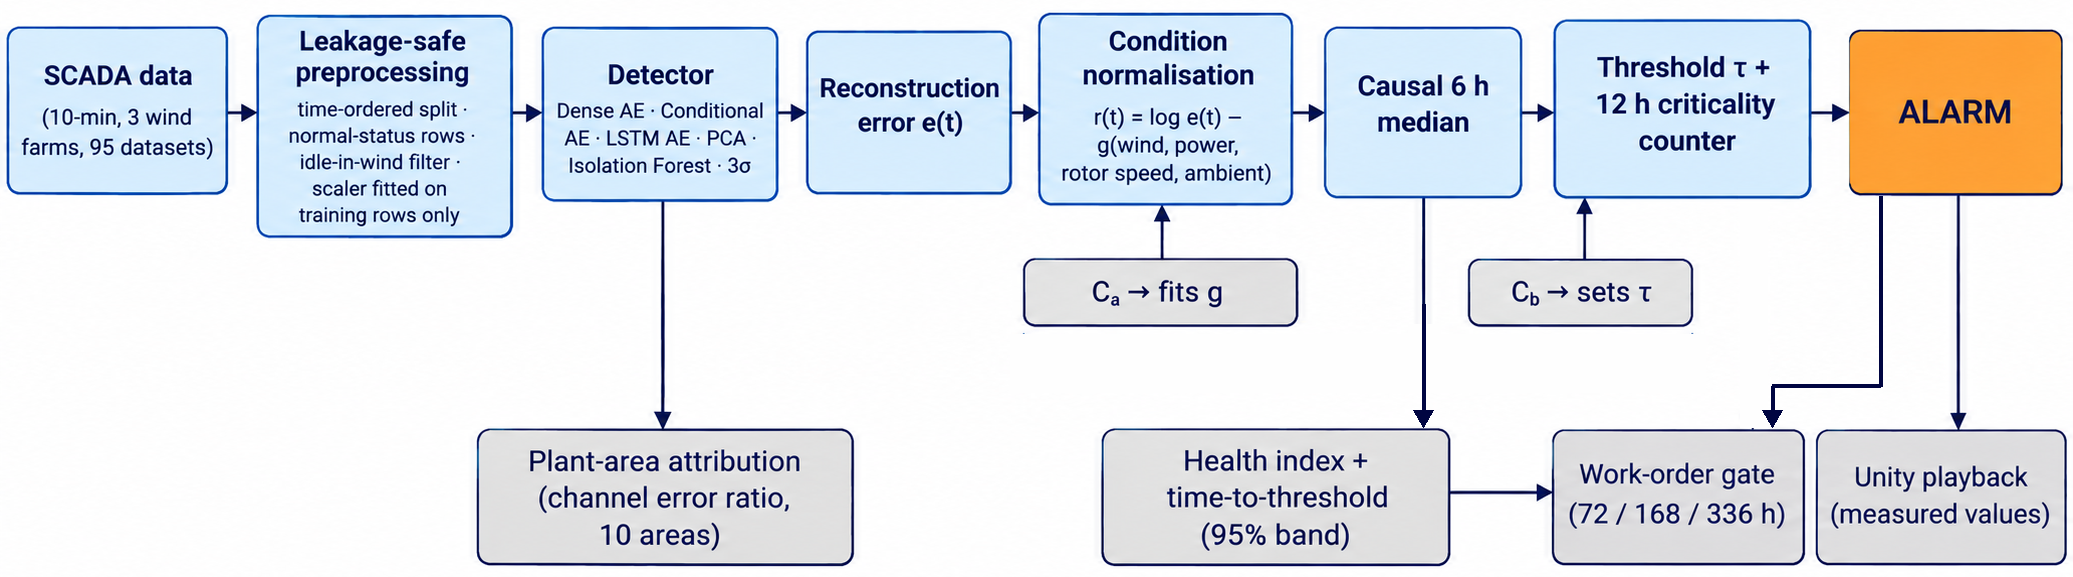
\includegraphics[width=0.95\textwidth]{figures/pipeline.png}}{\fbox{\parbox{0.9\textwidth}{\centering\vspace{1.5cm}\PH{Redraw Fig.~1: SCADA $\to$ preprocessing + training filter $\to$ AE ($d$-256-64-16) $\to$ error $\to$ condition normalisation (regressor on wind, power, rotor speed, ambient) $\to$ 6 h median $\to$ threshold + 12 h counter $\to$ alarm; side branches: plant-area attribution, health index + time-to-threshold band, Unity playback}\vspace{1.5cm}}}}
\caption{Pipeline. The detector is trained on normal rows only; the condition model and the threshold use two separate held-out slices.}
\label{fig:pipeline}
\end{figure*}

\section{Related Work}
SCADA-based condition monitoring is reviewed in \cite{r20}. Early normal behaviour models predicted one temperature from a few operating inputs and flagged large residuals \cite{r21,r22,r23}; later work added change-point detection to keep such models robust after component swaps \cite{r24}. Inputs that are physically coupled to the target improve the fit but can hide the fault \cite{r26}, a point that returns in our results. Deep models extend the idea to many channels \cite{r2,r4,r25}, and autoencoders treat a large reconstruction error as a sign that the current row does not look like healthy training rows \cite{r10,r11}.

The work closest to ours comes from the group that released CARE-to-Compare. ARCANA attributes an autoencoder anomaly to input features through a sparse correction of the input \cite{r17}; transfer learning lets a model trained on one turbine serve another \cite{r18}; and a conditional autoencoder worked well for district-heating substations \cite{r19}. The benchmark paper defines the CARE score and reports 0.66 for an autoencoder whose layer sizes, learning rate and thresholds were tuned per farm with Optuna, with an adaptive, error-predicting threshold on farms A and B, and 0.5 for random predictions \cite{r12}. Its earliness weighting follows the Numenta benchmark \cite{r27}. Our condition normalisation is a post-hoc relative of that adaptive threshold; the difference here is that nothing is tuned on the test data.

Digital-twin surveys rank implementations from a standalone 3D model up to an autonomous plant \cite{r7,r8}; structural twins estimate remaining life from load histories \cite{r14,r15}. The Unity scene here is a descriptive playback. Reporting follows the REFORMS checklist for machine-learning-based science \cite{r28}.

\section{Dataset}
CARE-to-Compare \cite{r12} holds 95 datasets from three farms (Table~\ref{tab:data}). Farm A is an onshore farm in Portugal with 86 columns; farms B and C are offshore farms in Germany with 257 and 957 columns. Each dataset covers one turbine and splits into about a year of training data and a prediction window of 4 to 98 days. The prediction window holds either a labelled event that ends in a fault or a normal period. Every row carries a status code; codes 0 and 2 count as normal operation. Sensor names are anonymised, but each farm publishes a plain description of every sensor, and most fault events carry a short operator note on the root cause. Farm A's status codes were derived from the fault logbook, so they are used to choose training rows but ignored in evaluation, as in the benchmark's reference code.

\begin{table}[t]
\caption{Datasets used (all of CARE-to-Compare)}
\label{tab:data}
\centering
\begin{tabular}{lcccc}
\toprule
Farm & Site & Columns & Fault events & Normal periods\\
\midrule
A & onshore & 86 & 12 & 10\\
B & offshore & 257 & 6 & 9\\
C & offshore & 957 & 27 & 31\\
\midrule
All & & & 45 & 50\\
\bottomrule
\end{tabular}
\end{table}

Leakage rules were fixed before any test result was seen. Models are fitted only on training-year rows with normal status. Following the benchmark paper, training rows where the wind is between 5 and 20~m/s but power is below 2\% of its training 99th percentile are also dropped, because a turbine standing still in good wind is not healthy behaviour \cite{r12}. The last 15\% of the remaining rows are held out and split in time into two calibration slices, $\mathcal{C}_a$ and $\mathcal{C}_b$. Row identifiers, asset identifiers and the status code are removed from the inputs. Angle channels, counter channels (cumulative energy), channels with over 30\% missing values in training and constant channels are dropped. Gaps up to one hour are forward-filled, the rest take the training median, and each channel is standardised on the training rows and clipped to $\pm10$.

\section{Method}
\subsection{Detectors}
The main detector is a fully connected autoencoder with widths $d\!\to\!256\!\to\!64\!\to\!16\!\to\!64\!\to\!256\!\to\!d$, ReLU hidden layers and a linear output, since standardised inputs are unbounded. Training uses Adam ($10^{-3}$), batches of 256 and at most 40 epochs, with early stopping after five epochs without improvement on the held-out rows; each dataset is run with seeds 0, 1 and 2. The score is the mean squared reconstruction error
\begin{equation}
e(t)=\tfrac{1}{d}\lVert \mathbf{x}(t)-\hat{\mathbf{x}}(t)\rVert_2^2 .
\end{equation}
Two variants test specific choices: the same network with a sigmoid output, which cannot reproduce negative standardised values, and a conditional autoencoder that receives the four scaled operating conditions both at its input and next to its 16-unit code \cite{r19}. Three baselines see the same rows: Isolation Forest with 200 trees \cite{r16}, PCA keeping 95\% of training variance, and the fraction of channels lying more than 3$\sigma$ from their training mean.

\subsection{Condition normalisation and smoothing}
Even on healthy rows, $e(t)$ depends on where the turbine is operating. Let $\mathbf{u}(t)$ hold wind speed, active power, rotor speed and ambient temperature. A histogram gradient-boosting regressor $g$ is fitted on slice $\mathcal{C}_a$, which the detector never trained on, to predict $\log e$ from $\mathbf{u}$. The normalised score is
\begin{equation}
r(t)=\log e(t)-g(\mathbf{u}(t)),
\end{equation}
the part of the error that the operating point does not explain. A causal 6-hour rolling median then removes isolated spikes. Every detector is reported raw, smoothed, normalised, and normalised plus smoothed, so the effect of each step can be read off directly.

\subsection{Thresholds and alarms}
A row is flagged when its score exceeds the 99th percentile of the same score on slice $\mathcal{C}_b$. Alarms use the benchmark's counter \cite{r12}: it rises by one on a flagged normal-status row, falls by one (not below zero) on a clean one, and holds on other statuses; an alarm is raised when it reaches 72, i.e.\ 12~h of net abnormal behaviour. These settings (Table~\ref{tab:settings}) are used for every main result. Separately, to measure what tuning is worth without touching the test farm, the quantile ($0.95$ to $0.999$) and the counter (36, 72, 144) are chosen on two farms and applied to the third, for each farm in turn.

\begin{table}[t]
\caption{Settings fixed before evaluation}
\label{tab:settings}
\centering
\setlength{\tabcolsep}{4pt}
\begin{tabular}{ll}
\toprule
Item & Setting\\
\midrule
Training filter & wind 5--20 m/s and power $<2\%$ of $P_{99}$ removed\\
Autoencoder & $d\to256\to64\to16\to64\to256\to d$, ReLU, linear out\\
Optimiser & Adam $10^{-3}$, batch 256, $\le40$ epochs, patience 5\\
Seeds & 0, 1, 2\\
Condition model & HistGBR, 200 trees, rate 0.05, on $\mathcal{C}_a$\\
Smoothing & causal rolling median, 6 h\\
Row threshold & 99th percentile on $\mathcal{C}_b$\\
Alarm & counter $\ge 72$ (12 h) \cite{r12}\\
Baselines & Isolation Forest \cite{r16}, PCA (95\%), 3$\sigma$ fraction\\
\bottomrule
\end{tabular}
\end{table}

\subsection{Evaluation}
The CARE score \cite{r12} combines four parts: coverage, a row-wise $F_{0.5}$ inside the labelled windows of fault datasets; accuracy, the share of rows left unflagged in normal datasets; reliability, an event-wise $F_{0.5}$ over all datasets based on the alarm counter; and earliness, a weighted share of flagged rows that favours the start of each window \cite{r27}. The score is $(\mathrm{Cov}+\mathrm{Earl}+\mathrm{Rel}+2\,\mathrm{Acc})/5$; it is 0 if nothing is detected and equals the accuracy if that falls to 0.5 or below. Our implementation follows the paper and, where the paper leaves a choice open, the authors' reference code. Abnormal-status rows are left out of coverage and accuracy. We also report how many faults were detected and how many normal periods raised an alarm, with 95\% Wilson intervals. Because the 95 datasets, not the three seeds, are the main source of variation, differences between two configurations are tested with a paired bootstrap that resamples fault and normal datasets separately (1000 draws) and recomputes both CARE scores on each draw.

\subsection{Plant-area attribution}
Each channel is assigned to one of ten plant areas (pitch and hub, yaw, hydraulics and brakes, cooling, gearbox, generator, rotor and drivetrain, nacelle and tower, electrical, environment) by ordered keyword rules on its published description. Over the labelled window, each channel's error is divided by its own mean error on the held-out rows, and areas are ranked in three ways fixed in advance: by the mean ratio, by the summed ratio, and by a vote of the ten highest-ratio channels. For ground truth, the authors read every operator note and assigned one or more areas to it; five vague notes (communication faults, unknown standstills) were left out, leaving 40 labelled faults. Rankings are scored by top-1 and top-3 hit rates against three floors: a random ranking, always naming the most common area (an oracle floor, since it peeks at the labels), and the same mean-ratio rule applied to the channels' absolute z-scores, which needs no model.

\subsection{Health index and time to threshold}
For the case studies, the normalised, smoothed score $\tilde r(t)$ is mapped to a health index using its median $q_{50}$ and 99th percentile $q_{99}$ on $\mathcal{C}_b$:
\begin{equation}
\mathrm{HI}(t)=\left(1+\frac{\max(0,\tilde r(t)-q_{50})}{q_{99}-q_{50}}\right)^{-1}.
\end{equation}
HI is one at typical healthy behaviour, 0.5 at the alarm threshold and falls towards zero beyond it, using no future data. The slope $s(t)$ is a least-squares fit of HI on time over the previous 24~h. The time to a floor $\mathrm{HI}_{th}=0.2$ is $\widehat T(t)=(\mathrm{HI}(t)-\mathrm{HI}_{th})/(-s(t))$ for $s(t)<0$, capped at 720~h, and $s\pm1.96\,\mathrm{SE}(s)$ gives a 95\% band. A work order is suggested when an alarm is active and $\widehat T$ falls below a gate $G$, with the visit a buffer $B$ earlier. Neither $G$ nor $B$ can be fitted without a maintenance log, so we report $G\in\{72,168,336\}$~h and $B\in\{12,24,48\}$~h as a sensitivity table instead of fixing them.

\subsection{Temperature model, robustness and playback}
As a supervised cross-check on farm C, a gradient-boosting model predicts rotor-bearing and generator cooling-water outlet temperatures from rotor speed, power, ambient temperature and wind speed (farm C has no humidity channel). It is trained on normal rows of dataset 44, tested on later rows of the same turbine and on another turbine (dataset 61), and compared with linear regression and a constant-mean floor; intervals come from a bootstrap over whole days. To probe sensor noise and dropouts, the prediction window of every dataset is corrupted with Gaussian noise ($\sigma=0.1,0.3,0.5$ in standardised units) or with 5\% and 20\% of entries replaced by the training median, and rescored by the autoencoder (seed 0) and PCA without retraining or moving the threshold. Finally, measured wind speed, rotor speed, power and temperatures are exported with the anomaly score, alarm, HI and $\widehat T$ band to a time-indexed CSV that drives a simplified Unity turbine.

\section{Results}
\subsection{Detection on 95 datasets}
Table~\ref{tab:care} gives the CARE score of every detector and post-processing step. With the fixed settings the plain autoencoder reaches 0.584, smoothing raises it to 0.595 and the full pipeline gives 0.592, all clearly above random (0.5) but below the tuned benchmark autoencoder (0.66) \cite{r12}. Condition normalisation on its own lowers the score to 0.568. It does what it was designed to do on healthy data, raising accuracy on normal periods from 0.962 to 0.970 and cutting alarms in normal periods from 5 to 4, but coverage drops from 0.24 to 0.20 and detected faults from 11.3 to 10.3. A likely reason is that part of the fault signal itself rises with load, so the regressor learns to expect it; this would be the input-coupling effect noted in \cite{r26}. The paired bootstrap confirms that none of these differences is reliable: smoothing over raw gives $+0.011$ (95\% CI $-0.018$ to $0.047$), normalisation over raw $-0.017$ ($-0.044$ to $0.009$), and the full pipeline over smoothing alone $-0.004$ ($-0.037$ to $0.025$). PCA does as well as the autoencoder (0.598 with both steps; difference $-0.007$, CI $-0.045$ to $0.032$). The post-processing matters more for weak detectors: Isolation Forest rises from 0.467 to 0.515 with both steps, the only significant gain ($+0.048$, CI $0.003$ to $0.094$), and the 3$\sigma$ rule from 0.482 to 0.520. The training filter is close to neutral (0.592 with and without it, one seed). The full pipeline detected 15.3 of 45 faults (95\% CI 0.21 to 0.48) and raised alarms in 7.0 of 50 normal periods (0.07 to 0.26), with a median first alarm 147~h before the end of the event window.

\begin{table}[t]
\caption{CARE score on all 95 datasets. AE rows: mean $\pm$ s.d.\ over three seeds. Det.: faults detected of 45; FA: normal periods with an alarm, of 50. Benchmark reference: tuned AE 0.66, random 0.5 \cite{r12}.}
\label{tab:care}
\centering
\setlength{\tabcolsep}{2.2pt}
\begin{tabular}{llcccccc}
\toprule
Detector & Post-proc. & CARE & Cov. & Acc. & Rel. & Det. & FA\\
\midrule
AE & raw & 0.584$\pm$.002 & 0.24 & 0.962 & 0.51 & 11.3 & 5.0\\
AE & + smooth & 0.595$\pm$.004 & 0.24 & 0.952 & 0.59 & 17.7 & 8.3\\
AE & + cond.\ norm. & 0.568$\pm$.003 & 0.20 & 0.970 & 0.50 & 10.3 & 4.0\\
AE & + both & 0.592$\pm$.004 & 0.26 & 0.953 & 0.57 & 15.3 & 7.0\\
AE, no filter & + both & 0.592 & 0.26 & 0.956 & 0.57 & 16 & 8\\
AE, sigmoid out & raw & \PH{} & \PH{} & \PH{} & \PH{} & \PH{} & \PH{}\\
Cond.\ AE & raw / both & \PH{} & \PH{} & \PH{} & \PH{} & \PH{} & \PH{}\\
Isol.\ Forest & raw & 0.467 & 0.11 & 0.982 & 0.14 & 2 & 5\\
Isol.\ Forest & + both & 0.515 & 0.15 & 0.977 & 0.38 & 9 & 9\\
PCA & raw & 0.595 & 0.25 & 0.963 & 0.54 & 10 & 2\\
PCA & + both & 0.598 & 0.29 & 0.936 & 0.55 & 16 & 9\\
3$\sigma$ fraction & raw & 0.482 & 0.11 & 0.979 & 0.21 & 4 & 9\\
3$\sigma$ fraction & + both & 0.520 & 0.14 & 0.982 & 0.43 & 8 & 4\\
\bottomrule
\end{tabular}
\end{table}

Per farm, the full pipeline scores 0.604 on A, 0.580 on B and 0.592 on C; it detects 5 of 12 faults on A with no alarm in A's normal periods, but only 8 of 27 on C, where it also raises 6.3 of the 7 false alarms. Pitch, hub-electronics and communication faults make up most of farm C's events, and many of them leave little trace in 10-minute averages, which agrees with a recent finding that 28 of the 45 benchmark faults sit in systems no temperature sensor watches.\footnote{\url{https://github.com/kwwaleszczynski-del/wind-thermal-nbm}}

\textit{What tuning is worth.} \PH{From lofo.csv: CARE with fixed settings vs leave-one-farm-out tuned settings for AE, conditional AE and PCA, the settings chosen per held-out farm, and the in-sample best as an optimistic ceiling. State how much of the 0.59 to 0.66 gap closes.} \PH{From counter\_sensitivity.csv: one sentence on counters 36 and 144.} \PH{From bootstrap.csv: conditional AE vs AE and vs post-hoc normalisation.} \PH{From val\_loss\_heads.csv: median best validation loss of the sigmoid head vs the linear head (linear: 0.196 in v2), and its CARE score.}

\subsection{Attribution against operator notes}
Table~\ref{tab:attribution} scores the ranking rules on the 40 labelled faults. Over all farms the vote rule names a correct area first in 37\% of faults and within the top three in 64\%, well above a random ranking (12\% and 35\%) but only level with always naming pitch and hub, the commonest area (30\% and 70\%). Per farm the picture is weaker. On farm C the summed and vote rules (47\% and 48\% top-1) fall short of always answering pitch (55\%), because pitch dominates the notes. On farm A no rule beats a random ranking at top-1 (8\%), while always answering hydraulics and brakes gives 50\%; farm B's six faults (transformer and rotor bearing) are too few to separate the rules from the floor. \PH{v3: the model-free $|z|$ rule against the AE rules.} Attribution therefore narrows the search, but it is not yet better than an operator's prior about which area usually fails.

\begin{table}[t]
\caption{Top-$k$ hit rate of plant-area attribution over 40 labelled faults (AE rules: mean over three seeds)}
\label{tab:attribution}
\centering
\begin{tabular}{lcc}
\toprule
Rule & Top-1 & Top-3\\
\midrule
Mean ratio & 0.33 & 0.62\\
Summed ratio & 0.36 & 0.66\\
Top-10 channel vote & 0.37 & 0.64\\
$|z|$ ratio, no model & \PH{} & \PH{}\\
Random ranking & 0.12 & 0.35\\
Most common area (oracle) & 0.30 & 0.70\\
\bottomrule
\end{tabular}
\end{table}

\subsection{Case studies: a missed and a detected fault}
The operator note for dataset 44 (farm C) reads ``valve in water cooling system was left in wrong position after maintenance''. The pipeline did not detect it: only 20 of 8788 rows in the window crossed the threshold, no alarm fired, and the window-level ROC-AUC was 0.67 (Fig.~\ref{fig:hi}). Consequently no work order is raised at any gate (Table~\ref{tab:gate}). Attribution was still informative: over the labelled window the cooling area ranked first of ten, with a mean error ratio of 1.82 against 1.57 for the next area (Fig.~\ref{fig:rca}). \PH{v3, dataset 40 (farm A, generator bearing): first alarm relative to the event start, rank of the generator area, $\widehat T$ band width and gate triggers (Fig.~\ref{fig:ttt}, Table~\ref{tab:gate}).}

\begin{figure}[t]
\centering
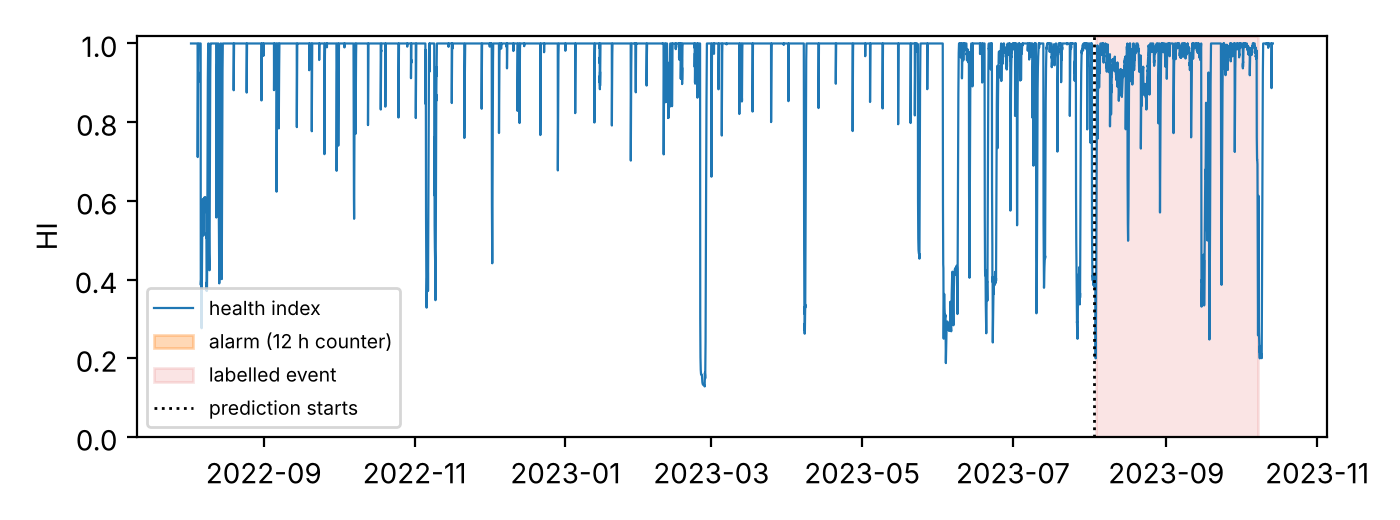
\includegraphics[width=\columnwidth]{figures/fig_hi_44.png}
\caption{Health index for dataset 44 with alarm periods (none) and the labelled event (shaded).}
\label{fig:hi}
\end{figure}

\begin{figure}[t]
\centering
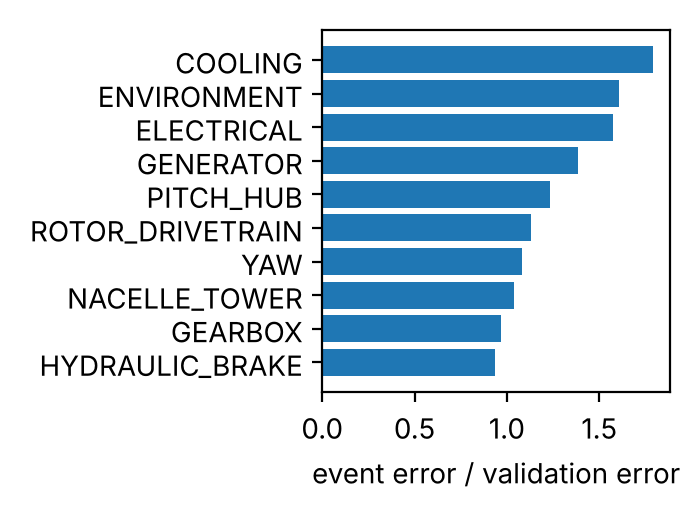
\includegraphics[width=0.85\columnwidth]{figures/fig_rca_44.png}
\caption{Plant-area attribution over the labelled window of dataset 44.}
\label{fig:rca}
\end{figure}

\begin{figure}[t]
\centering
\IfFileExists{figures/fig_ttt_40.png}{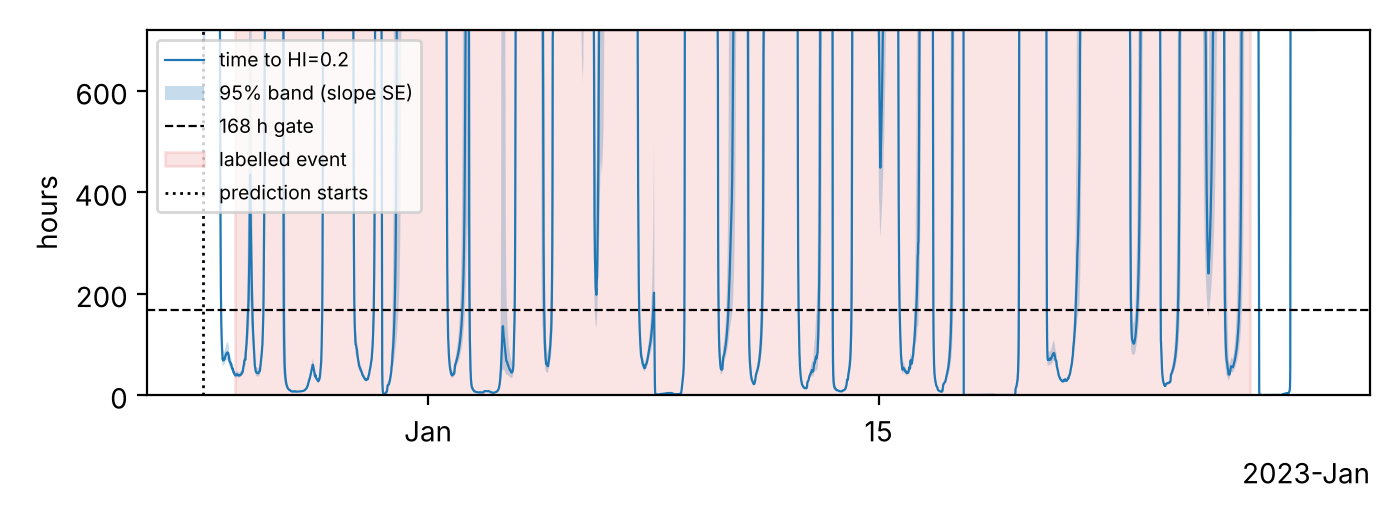
\includegraphics[width=\columnwidth]{figures/fig_ttt_40.png}}{\fbox{\parbox{0.9\columnwidth}{\centering\PH{fig\_ttt\_40.png from v3}}}}
\caption{Time to $\mathrm{HI}=0.2$ for dataset 40 with a 95\% band from the slope standard error.}
\label{fig:ttt}
\end{figure}

\begin{table}[t]
\caption{Gate sensitivity (first work-order trigger, hours relative to event start; $B$=24 h)}
\label{tab:gate}
\centering
\begin{tabular}{ccccc}
\toprule
Gate $G$ & \multicolumn{2}{c}{Dataset 44} & \multicolumn{2}{c}{Dataset 40}\\
 & First trigger & Triggers in $\mathcal{C}_b$ & First trigger & Triggers in $\mathcal{C}_b$\\
\midrule
72 & none & 0 & \PH{} & \PH{}\\
168 & none & 0 & \PH{} & \PH{}\\
336 & none & 0 & \PH{} & \PH{}\\
\bottomrule
\end{tabular}
\end{table}

\subsection{Temperature model and robustness}
Table~\ref{tab:temp} gives the temperature hold-out scores on farm C. Gradient boosting explains about 58\% of the variance of rotor-bearing temperature on later rows of the same turbine (MAE 2.3~$^\circ$C) but only 21\% on turbine 61, where a linear model does better ($R^2=0.30$); for cooling-water outlet temperature it reaches $R^2$ of 0.31 and 0.27 with MAE of 1.4 and 1.0~$^\circ$C, against a constant-mean floor with negative $R^2$. During the valve fault the mean residual of cooling-water outlet temperature moved from $-0.64$~$^\circ$C on held-out healthy rows to $0.00$~$^\circ$C (Fig.~\ref{fig:temp}), a shift well inside the model's error, which is consistent with the missed detection. \PH{v3, from robustness.csv: CARE, detected faults and false alarms of AE and PCA under noise up to $\sigma=0.5$ and 20\% missing entries, against the clean scores.}

\begin{table}[t]
\caption{Temperature model, gradient boosting (95\% day-block bootstrap CI)}
\label{tab:temp}
\centering
\setlength{\tabcolsep}{3pt}
\begin{tabular}{llcc}
\toprule
Target & Test set & MAE ($^\circ$C) & $R^2$\\
\midrule
Rotor bearing & same turbine, later & 2.32 [1.87, 2.83] & 0.58 [0.46, 0.67]\\
Rotor bearing & turbine 61 & 2.39 [2.26, 2.53] & 0.21 [0.14, 0.28]\\
Cooling water out & same turbine, later & 1.43 [1.02, 1.89] & 0.31 [0.18, 0.41]\\
Cooling water out & turbine 61 & 1.03 [0.94, 1.14] & 0.27 [0.13, 0.38]\\
\bottomrule
\end{tabular}
\end{table}

\begin{figure}[t]
\centering
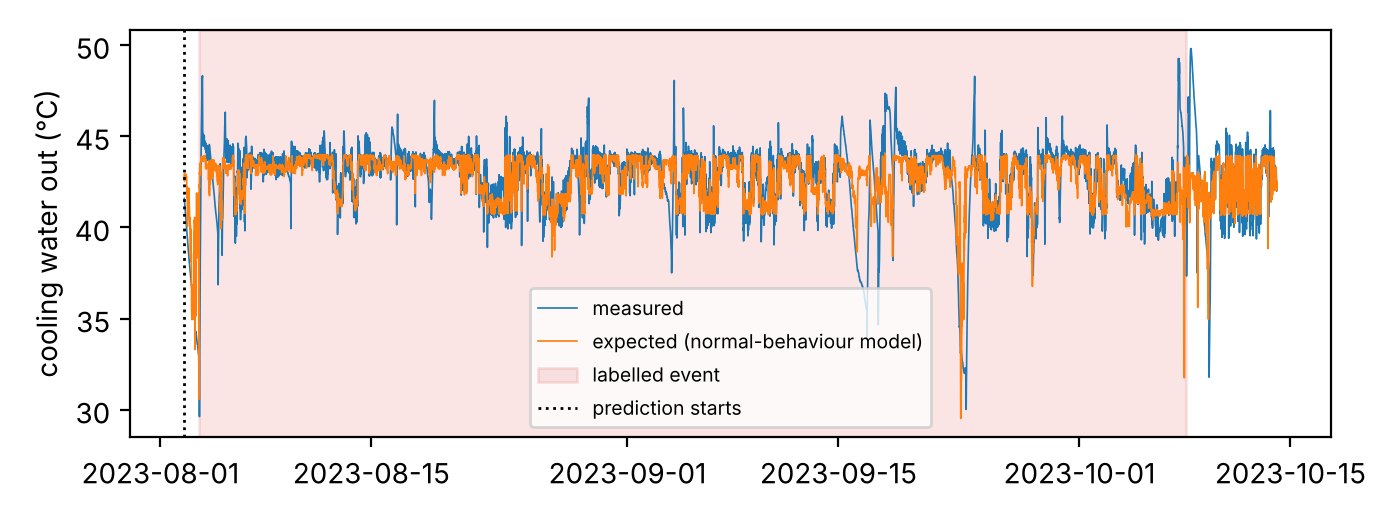
\includegraphics[width=\columnwidth]{figures/fig_temp_44.png}
\caption{Measured and expected generator cooling-water outlet temperature in the prediction window of dataset 44.}
\label{fig:temp}
\end{figure}

\subsection{Playback and scope}
Fig.~\ref{fig:unity} is a frame from the Unity scene. Every value on screen is a measured SCADA reading or a model output for that time stamp; the scene is a briefing view, not evidence that the model is correct. Table~\ref{tab:scope} places the work against published SCADA and twin papers.

\begin{figure}[t]
\centering
\IfFileExists{figures/warning.png}{\includegraphics[width=\columnwidth]{figures/warning.png}}{\fbox{\parbox{0.9\columnwidth}{\centering Unity frame goes here}}}
\caption{Unity playback of one sample from dataset 44. \PH{re-export the frame from unity\_telemetry\_44.csv}}
\label{fig:unity}
\end{figure}

\begin{table}[t]
\caption{Scope against selected prior papers}
\label{tab:scope}
\centering
\setlength{\tabcolsep}{3pt}
\begin{tabular}{lcccccc}
\toprule
Work & Bench. & AD & RCA & Life & Plan & Twin\\
\midrule
Lee et al.\ \cite{r2} & no & yes & no & no & no & no\\
Encalada et al.\ \cite{r11} & no & yes & no & no & no & no\\
Roelofs et al.\ \cite{r17} & no & yes & yes & no & no & no\\
G\"uck et al.\ \cite{r12} & yes & yes & no & no & no & no\\
Stadtmann et al.\ \cite{r13} & no & yes & yes & no & no & yes\\
This paper & yes & yes & checked & est. & yes & play.\\
\bottomrule
\end{tabular}
\end{table}

\section{Discussion and Limits}
\textit{Why normalisation did not help the autoencoder.} The regressor removes whatever the operating point predicts, and on these turbines part of the fault signal is itself load-dependent. Normalisation trades coverage for accuracy, and the CARE score, which weights accuracy twice, ends up roughly where it started. Weak detectors whose errors are dominated by operating point, such as Isolation Forest, gain the most.

\textit{What the score can and cannot see.} Ten-minute averages smooth away short electrical and communication faults, and some pitch faults only show in signals that are not logged. No change to the detector can recover information that the data do not contain.

\textit{Life figure.} $\widehat T$ is a short-horizon slope to a chosen floor. The benchmark publishes no component replacement times, so no remaining-useful-life error can be computed, and the band covers slope noise only.

\textit{Attribution labels.} Plant areas were assigned to operator notes by the authors. The notes are brief and several faults involve more than one area.

\textit{Deployment.} Communication loss, vessel delay and weather lock-outs sit outside the CSV, and the robustness test covers noise and dropouts in the signal only. The gate and buffer are left to the operator.

\textit{Playback twin.} The Unity scene reads a CSV. It does not close a loop with the plant and does not host a physics model.

\section{Conclusion}
On all 95 CARE-to-Compare datasets, with settings fixed in advance, a dense autoencoder reaches a CARE score of 0.584, and condition normalisation and causal smoothing move it by less than the variation between datasets; PCA does as well. Normalisation lowers false alarms but also hides load-dependent fault signal, and it pays off only for weaker detectors such as Isolation Forest. \PH{One sentence on leave-one-farm-out tuning and the conditional AE.} Plant-area attribution beats a random ranking clearly but only matches always naming the commonest area. The cooling-valve fault was missed although the cooling area ranked first, and the time-to-threshold band remains a planning aid rather than a fitted life model. Next steps are fitting the gate to a real maintenance log and transferring the condition model between turbines \cite{r18}.

\begin{thebibliography}{29}
\bibitem{r1} A. Tavares and M. Giesbrecht, ``Deep Learning-Based Fault Diagnosis in Wind Turbine Bearings and Gearboxes Using Vibration Signals,'' \textit{IEEE Access}, 2025, doi: 10.1109/ACCESS.2025.3636831.
\bibitem{r2} Y. Lee, C. Park, N. Kim, J. Ahn, and J. Jeong, ``LSTM-Autoencoder Based Anomaly Detection Using Vibration Data of Wind Turbines,'' \textit{Sensors}, vol. 24, no. 9, Art. no. 2833, 2024.
\bibitem{r3} L. Cummins \textit{et al.}, ``Explainable Predictive Maintenance: A Survey of Current Methods, Challenges and Opportunities,'' \textit{IEEE Access}, vol. 12, pp. 57574--57602, 2024.
\bibitem{r4} Y. Wang, Y. Zhao, and S. Addepalli, ``Remaining Useful Life Prediction using Deep Learning Approaches: A Review,'' \textit{Procedia Manuf.}, vol. 49, pp. 81--88, 2020.
\bibitem{r5} M. Achouch \textit{et al.}, ``On Predictive Maintenance in Industry 4.0: Overview, Models, and Challenges,'' \textit{Appl. Sci.}, vol. 12, no. 16, p. 8081, 2022.
\bibitem{r6} A. Haghshenas, ``Predictive Digital Twin of Wind Farm,'' M.S. thesis, NTNU, 2022.
\bibitem{r7} F. Stadtmann \textit{et al.}, ``Digital Twins in Wind Energy: Emerging Technologies and Industry-Informed Future Directions,'' \textit{IEEE Access}, vol. 11, pp. 110762--110795, 2023.
\bibitem{r8} E. Kandemir, A. Hasan, T. Kvamsdal, and S. A. Alaliyat, ``Predictive digital twin for wind energy systems: A literature review,'' \textit{Energy Informat.}, vol. 7, Art. no. 68, 2024.
\bibitem{r9} C. Tsallis, P. Papageorgas, D. Piromalis, and R. A. Munteanu, ``Application-Wise Review of Machine Learning-Based Predictive Maintenance,'' \textit{Appl. Sci.}, vol. 15, no. 9, p. 4898, 2025.
\bibitem{r10} A. Gonz\'alez-Mu\~niz, I. D\'iaz, A. A. Cuadrado, and D. Garc\'ia-P\'erez, ``Health indicator for machine condition monitoring built in the latent space of a deep autoencoder,'' \textit{Reliab. Eng. Syst. Saf.}, vol. 224, p. 108482, 2022.
\bibitem{r11} A. Encalada-D\'avila, C. Tutiv\'en, B. Puruncajas, and Y. Vidal, ``Wind turbine multi-fault detection based on SCADA data via an AutoEncoder,'' \textit{Renew. Energy Power Qual. J.}, vol. 19, pp. 487--492, 2021.
\bibitem{r12} C. G\"uck, C. M. A. Roelofs, and S. Faulstich, ``CARE to Compare: A Real-World Benchmark Dataset for Early Fault Detection in Wind Turbine Data,'' \textit{Data}, vol. 9, no. 12, p. 138, 2024.
\bibitem{r13} F. Stadtmann and A. Rasheed, ``Diagnostic Digital Twin for Anomaly Detection in Floating Offshore Wind Energy,'' arXiv:2406.02775, 2024.
\bibitem{r14} R. Pacheco-Blazquez, J. Garcia-Espinosa, D. Di Capua, and A. Pastor Sanchez, ``A Digital Twin for Assessing the Remaining Useful Life of Offshore Wind Turbine Structures,'' \textit{J. Mar. Sci. Eng.}, vol. 12, no. 4, Art. no. 573, 2024.
\bibitem{r15} A. Pastor-Sanchez \textit{et al.}, ``Real-Time Digital Twin for Structural Health Monitoring of Floating Offshore Wind Turbines,'' \textit{J. Mar. Sci. Eng.}, vol. 13, no. 10, Art. no. 1953, 2025.
\bibitem{r16} F. T. Liu, K. M. Ting, and Z.-H. Zhou, ``Isolation Forest,'' in \textit{Proc. IEEE Int. Conf. Data Mining (ICDM)}, 2008, pp. 413--422.
\bibitem{r17} C. M. A. Roelofs, M.-A. Lutz, S. Faulstich, and S. Vogt, ``Autoencoder-based anomaly root cause analysis for wind turbines,'' \textit{Energy and AI}, vol. 4, Art. no. 100065, 2021, doi: 10.1016/j.egyai.2021.100065.
\bibitem{r18} C. M. A. Roelofs, C. G\"uck, and S. Faulstich, ``Transfer learning applications for autoencoder-based anomaly detection in wind turbines,'' \textit{Energy and AI}, vol. 17, Art. no. 100373, 2024, doi: 10.1016/j.egyai.2024.100373.
\bibitem{r19} C. M. A. Roelofs, E. Guevara Bastidas, T. Hugo, S. Faulstich, and A. Cadenbach, ``Enabling predictive maintenance in district heating substations: A labelled dataset and fault detection evaluation framework based on service data,'' \textit{Energy}, vol. 355, Art. no. 141178, 2026, doi: 10.1016/j.energy.2026.141178.
\bibitem{r20} J. Tautz-Weinert and S. J. Watson, ``Using SCADA data for wind turbine condition monitoring -- a review,'' \textit{IET Renew. Power Gener.}, vol. 11, no. 4, pp. 382--394, 2017, doi: 10.1049/iet-rpg.2016.0248.
\bibitem{r21} A. Zaher, S. D. J. McArthur, D. G. Infield, and Y. Patel, ``Online wind turbine fault detection through automated SCADA data analysis,'' \textit{Wind Energy}, vol. 12, no. 6, pp. 574--593, 2009, doi: 10.1002/we.319.
\bibitem{r22} M. Schlechtingen and I. F. Santos, ``Wind turbine condition monitoring based on SCADA data using normal behavior models. Part 2: Application examples,'' \textit{Appl. Soft Comput.}, vol. 14, pp. 447--460, 2014, doi: 10.1016/j.asoc.2013.09.016.
\bibitem{r23} P. Bangalore and L. B. Tjernberg, ``An artificial neural network approach for early fault detection of gearbox bearings,'' \textit{IEEE Trans. Smart Grid}, vol. 6, no. 2, pp. 980--987, 2015, doi: 10.1109/TSG.2014.2386305.
\bibitem{r24} S. Letzgus, ``Change-point detection in wind turbine SCADA data for robust condition monitoring with normal behaviour models,'' \textit{Wind Energy Sci.}, vol. 5, pp. 1375--1397, 2020, doi: 10.5194/wes-5-1375-2020.
\bibitem{r25} G. Helbing and M. Ritter, ``Deep learning for fault detection in wind turbines,'' \textit{Renew. Sustain. Energy Rev.}, vol. 98, pp. 189--198, 2018, doi: 10.1016/j.rser.2018.09.012.
\bibitem{r26} T. Felgueira, S. Rodrigues, C. S. Perone, and R. Castro, ``The impact of feature causality on normal behaviour models for SCADA-based wind turbine fault detection,'' arXiv:1906.12329, 2019.
\bibitem{r27} A. Lavin and S. Ahmad, ``Evaluating real-time anomaly detection algorithms -- the Numenta Anomaly Benchmark,'' in \textit{Proc. IEEE 14th Int. Conf. Mach. Learn. Appl. (ICMLA)}, 2015, pp. 38--44, doi: 10.1109/ICMLA.2015.141.
\bibitem{r28} S. Kapoor \textit{et al.}, ``REFORMS: Consensus-based recommendations for machine-learning-based science,'' \textit{Sci. Adv.}, vol. 10, no. 18, Art. no. eadk3452, 2024, doi: 10.1126/sciadv.adk3452.
\bibitem{r29} R. R. Nair, T. Babu, A. Panthakkan, B. Balusamy, and W. Mansoor, ``Hybrid autoencoder-based framework for early fault detection in wind turbines,'' arXiv:2510.15010, 2025.
\end{thebibliography}

\end{document}
